\chapter{Charts and Tables}
\section{Skill Roll Outcome Graph}
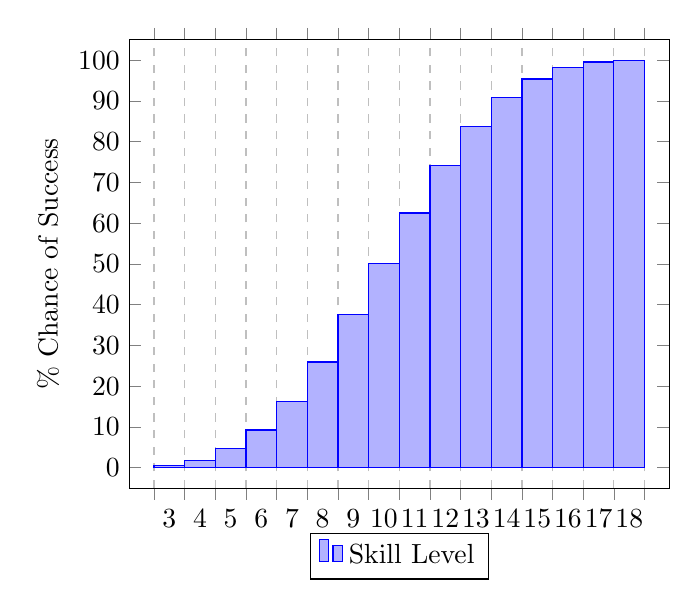
\begin{tikzpicture}
\begin{axis}[
	x tick label style={/pgf/number format/1000 sep=},
	ylabel=\% Chance of Success,
	enlargelimits=0.05,
	ytick = {0, 10, 20, 30, 40, 50, 60, 70, 80, 90, 100},
	legend style = {
	    at={(0.5,-0.1)},
	    grid style = dashed,
	    anchor=north,legend columns=-1
	},
	ybar interval = 1,
]
\addplot 
	coordinates {
	    (3,    0.46) 
	    (4,    1.85)
		(5,    4.63) 
		(6,    9.26) 
		(7,   16.20) 
		(8,   25.93) 
		(9,   37.50) 
		(10,  50.00) 
		(11,  62.50) 
		(12,  74.07)
		(13,  83.80)
		(14,  90.74)
		(15,  95.37)
		(16,  98.15)
		(17,  99.54)
		(18, 100.00)
		(19, 0)
	};
\legend{Skill Level}
\end{axis}
\end{tikzpicture}\\
The graph above shows the probability of succeeding a skill roll. If your character has an effective skill of 10, they have a 50\% chance of succeeding that roll. If they have a skill of 12, the chance of success goes up to 74\%.
\section{Critical Miss Table (Melee)}
\begin{center}
\begin{tabular}{r | l}
    \textbf{Roll} & \textbf{Result}\\\hline
    1 & Your weapon turns in your hand, and you hit with the flat side! \\
    2 & Your weapon breaks! \\
    3 & You lose your grip and the weapon flies out of your hand! \\
    4 & You lose your balance, and your turn! \\
    5 & You trip and fall! You have to get up again.\\
    6 & You hit yourself in the arm or leg! (50\% chance of hitting either)\\
\end{tabular}
\end{center}
\paragraph{Note}For \#3, the weapon flies 1d6 squares (50\% chance forward or backward). If it hits someone, it does half damage and lands there.

%% \section{Critical Miss Table (Ranged)}
%% \begin{center}
%% \begin{tabular}{r | l}
%%     \textbf{Roll} & \textbf{Result}\\\hline
%%     1 & Your weapon jams.\\
%%     2 &\\
%%     3 &\\
%%     4 &\\
%%     5 &\\
%%     6 &\\
%% \end{tabular}
%% \end{center}

\section{Weapons} \label{sec:weapons}
\subsection{Melee Weapons}
\begin{center}
\begin{tabular}{c|c|c|c|c|c}
    \textbf{Category} & \textbf{Name} & \textbf{Class} & \textbf{Damage} & \textbf{Damage Type} & \textbf{Range} \\\hline
    Unarmed  & Fists          & Light & d6-2 & Crushing & Close/1\\
             & Feet           & Light & d6-1 & Crushing & Close/1\\\hline
    Medieval & Short Sword    & Light & d6   & Slashing & Close/1\\
             & Long Sword     & Heavy & d6+2 & Slashing & 1 to 2 \\
             & Mace           & Heavy & d6+2 & Crushing & Close/1\\\hline
    Modern   & Baseball Bat   & Heavy & d6+1 & Crushing & Close/1\\
             & Aluminium Bat  & Light & d6+1 & Crushing & Close/1\\
             & Brass Knuckles & Light & d6-1 & Crushing & Close/1\\\hline
    Future   & Beam Sword     & Light & d6+3 & Slashing & Close/1
\end{tabular}
\end{center}

\subsection{Ranged Weapons}
\begin{center}
\begin{tabular}{c|c|c|c|c}
    \textbf{Category} & \textbf{Name} & \textbf{Damage} & \textbf{Damage Type} & \textbf{Accurate Range} \\\hline
    Primitive & Rock        & d6-1  & Crushing & $0.5 \times Shooting + Prof$  \\\hline
    Medieval  & Short Bow   & d6+1  & Piercing & $Shooting + Prof$ \\
              & Long Bow    & d6+2  & Piercing & $2 \times Shooting + Prof$ \\\hline
    Modern    & Pistol      & 2d6+2 & Crushing & 56m \\
              & Shotgun     & 5d6   & Crushing & 3m \\\hline
    Future    & Laser Gun   & 6d6   & Piercing & 66m \\
\end{tabular}
\end{center}
\paragraph{Note} These ranges are for when you want to shoot without a range penalty.
So despite the fact that a pistol can shoot around 1800m, it's incredibly hard to do so.

\section{Armour}
\begin{center}
\begin{tabular}{c|c|c|c}
\textbf{Category} & \textbf{Name}  & \textbf{PD} & \textbf{DR}\\\hline
         Medieval & Learther       & 1 & 1 \\
                  & Half Plate     & 2 & 2 \\
                  & Full Plate     & 4 & 3 \\
                  & Chain Mail     & 1 & 1 \\\hline
           Modern & Summer Clothes & 0 & 0 \\
                  & Winter Clothes & 0 & 1 \\
                  & Kevlar Vest    & 1 & 3 \\\hline
           Future & Polymer        & 4 & 3 \\
\end{tabular}
\end{center}